\section{Narrative Roulette}

\emph{Narrative Roulette} (NR) is a microworld that does not require
students to learn a new language before being able to fully explore it.
Instead of being built around a programming language like Lisp,
\emph{Narrative Roulette} is built around a natural language: English.

You can find NR online at \url{http://kg.narrativeroulette.com}.

Rounds of \emph{Narrative Roulette} go like this: 

\begin{enumerate}
\item The teacher selects an interesting perspective for students to take. For example:
``You are the captain of a sinking ship''. 
\item Students have 15 minutes to write a few fictional, anonymous paragraphs from that perspective. 
\item After those 15 minutes are up, students read each other's
submissions and discuss them.
\item Then the teacher selects a new perspective and the next round begins. 
\end{enumerate}

\begin{figure}[ht!]
\centering
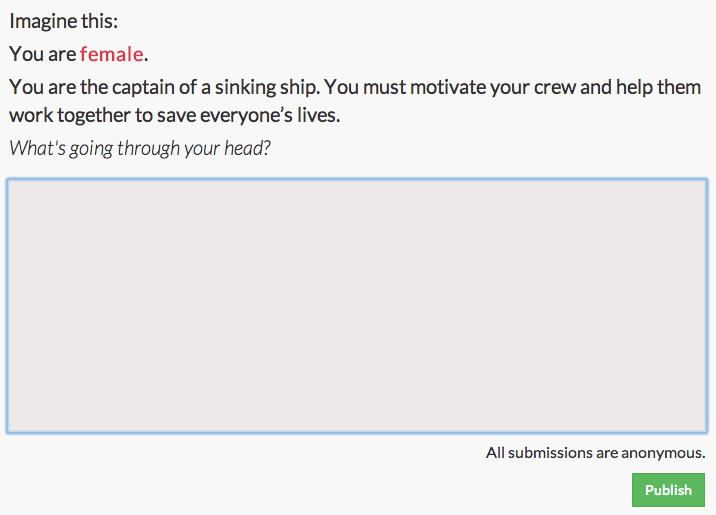
\includegraphics[width=115mm]{img/narrative_editor.png}
\caption{The Narrative Roulette microworld interface}
\label{overflow}
\end{figure}

\subsection{The benefits of being virtual}

As we can see, NR is a creative writing microworld. However, it is also
virtual and browser-based. Students read and write their texts in the
web browser, and discussions are had while reading texts from screens.

This allows the software to do all of the clerical work. Submissions are
edited by students using a web frontend, and then accepted and filed by
the backend. As the frontend does not send any identifying information
to the backend, anonymity is guaranteed. When it comes to letting
students read each other's work, the backend takes care of sending a
copy of each text to each student that requests one.

Without this custom-built software, students would have to write by
hand, and hope their handwriting is not recognisable by their peers or
their teacher. The teacher would have to accept submissions on paper,
photocopy them, and then hand them out to the class. This would waste
both paper and time, and result in lower motivation for the students.

\subsection{Narrative Roulette as a microworld}

Let's look at this round definition compared to an iteration of the
microworld loop: 

\begin{enumerate}
\item Students come up with \textbf{ideas} of what it would like to be the person in the situation named by the perspective.
\item Students \textbf{implement} their ideas in fictional texts. 
\item Students \textbf{evaluate} those texts by hearing what their peers think
of them.
\end{enumerate}

\emph{Narrative Roulette} is more directed than \emph{Talking to
Machines} (TTM). TTM was completely open-ended, allowing the student to
draw whatever they wished, whereas NR asks you to write from a
particular perspective.

This does not seem to have been a problem; in fact, it seems to have
helped focus the imaginations of the students taking part. A totally
blank canvas can be intimidating. A frame, such as ``you are the captain
of a sinking ship'', can help you start by providing a trigger for your imagination.

\subsection{How do you explore this microworld?}

Let's see how this works in practice.

A narrative in \emph{Narrative Roulette} contains characters, actions
and reactions. Narratives are written from the first-person perspective,
so a major character is the narrator, who is the character defined by
the round.

Texts usually take the form of internal monologue. This gives the reader
first-hand insight into the mental processes of the main character. It
also allows the writer to identify, examine and play around with the
mental processes they believe the main character could be having.

These mental processes lead to actions, or actually the narrator's
description of their actions. For example, the captain of a sinking ship
can decide to tell her crew that they need to get into a lifeboat. From
our vantage point, inside the narrator's mind, we can see \emph{why} she
does this: is she trying to help everyone on board, or is she getting
herself and the crew off the ship and leaving the passengers to die? The
writer gets to decide exactly how the narrator's thoughts manifest in
actions.

Consequences in the narrative are also chosen by the writer. Characters
react to the actions of the main character. The writer has to decide
what those reactions are; how they manifest in the actions of those
other characters; how the main character \emph{infers} these reactions
from the other characters' actions; and finally how the main character
reacts to all of these consequences.

And then there are the writer-defined constraints of the storyworld.
When we imagine a sinking ship, most of us would imagine enough
lifeboats to evacuate all the passengers and the crew. We are in control
of the storyworld, so why wouldn't we dream up circumstances in which
everyone gets saved?

Because in the real world, things don't always work out so nicely. It's
quite possible that there will be fewer seats on the lifeboats than
passengers and crew on the boat. Writers who want to challenge
themselves will realise this, and in their storyworlds, some people will
be left behind. The ensuing moral dilemma will be interesting to both
read and write about.

In essence, this is the difference between reading and writing text.
When you write, you have to make choices. You choose who your characters
are, how they behave and what consequences they have to deal with. Not
only this, but you also have to choose how you want to convey all of
this to the reader. When time and space is limited, as in
\emph{Narrative Roulette}, the best strategy is to say as much as
possible using the fewest words.

To recap, writers explore the \emph{Narrative Roulette} microworld by
\textbf{implementing} their \textbf{ideas} about characters, 
situation and behaviour in effective English prose.

\subsection{Why is this worth doing?}

Narrative theorists have said that the reason we read fiction is to gain
a better understanding of the psychologies of the main characters, from
their description in the text\cite{zunshine}. We read to learn about why
people act the way they do, by analysing fictitious characters and
situations. This exercises our theory of mind - our capacity to intuit
what other people are thinking and how they will behave.

Reading fiction is a worthwhile activity because the more accurate our
theory of mind, the better we are at understanding and predicting the
thoughts, feelings and behaviour of others and even ourselves.

When we \emph{write} fiction, we have to \textbf{construct} characters,
situations, actions, reactions, dialogue and description. In each of
these domains, we come up with \textbf{ideas}, \textbf{implement} them in
words, and then \textbf{evaluate} them by reading back our text as we
are writing it.

According to the constructionist learning theory, this means that we
\textbf{learn} about characters, situations, actions, reactions, dialogue and
description, by \textbf{constructing personal knowledge} about them. 

Learning how to write rounded characters means learning
about human psychology. Learning how to write characters' behaviour
means learning about human behaviour. Learning about how to construct
interesting situations means understanding the interplay between people
and their social, physical, cultural and emotional environment, and
being able to manipulate that interplay in the most interesting way.

Writing fiction is an exercise in constructing psychologies, situating
them in a storyworld, and then putting them through a chain of events
that make up a narrative. This means that a creative writing microworld
rewards (and thus improves) theory of mind as well as intuitive theories
of causation.

The very best fiction involves realistic characters dealing with
realistic consequences. Creative writing microworlds help students
construct knowledge about human nature and the world we live in.

\subsection{How are these texts evaluated?}

Criticising fictional texts is hard, we can see that much from the
disagreement that often surrounds literary criticism. One person's
favourite character might be the least favourite of another, and so on.
This makes it difficult for a single teacher, or any single
grade-setter, to pass judgement on a work of fiction.

In \emph{Narrative Roulette}, the entire readership of a work passes
judgement on a work. Currently, they do this by reading each other's
work in groups, and discussing them. The software can track how many
times a work has been read. In the future, the software will allow
readers to signal that they like a work, and to share it.

This allows for many dimensions in which works can be evaluated. A work of
fiction that no-one reads is a failure on a functional level - texts
exist to be read, so if no-one reads a text, it failed at what it was
meant to do. We could call texts that no-one reads \emph{valueless}.

Some texts will cause controversy. This means that the texts are read
and then fiercely debated. Sometimes, debaters will not approve of the
text. But the fact that the debaters read it, and then found things in
the text worthy of discussion, means that the text has some value.

Other texts will be liked by the majority of readers. This does not
necessarily make them \emph{better} than the more controversial works.
But near universal reader approval is still a form of success, as it means
that many people read the work. As with the controversial texts, the fact
that people read the work, and found things in the text worthy of
liking, means the text has value.

In this way, texts are primarily evaluated on their \emph{readability},
by the reading behaviour of other students - the writer's peers. This
can be called a \emph{structural} evaluation of a student's writing: how
good they are at communicating their ideas to their peers through the medium of
natural language.

The \emph{content} of a student's writing is evaluated by how much
discussion it generates, and how many people are willing to share it and like it.
Review-style comments (``I liked this part, but not this part'') count
as discussion.

This means that the traditional way of evaluating student's texts, where a
teacher writes a review (with an accompanying
grade), is just one component of a work's overall evaluation in the 
\emph{Narrative Roulette} microworld, instead of being the single authoritative evaluation as before. This makes a teacher's (or grade-setter's)
opinion less important. If a teacher considers a work of low value, but
the writer's peers all read, share and discuss it, the work will have high value
\emph{despite what the teacher thinks}.

This makes evaluation more democratic, and more like real-life. At school, a teacher or other authority's opinion of work has the power to
negatively affect a student's future: ``If you don't write your essay
using this exact structure, you'll get a bad grade, and not be able to
go to the university you want to.'' But after leaving school, the \emph{functional value} of work becomes all-important: ``If people don't read
your articles, we won't make money from ads on them, so you won't have a job at this company.'' Which
means that \emph{Narrative Roulette}'s form of evaluation is better
preparation for real-life than the evaluation methods of traditional school.

\subsection{How anonymity helps}

If the behaviour of peers dictates the evaluation of a work, won't
evaluation descend into a popularity contest? Won't students only read,
discuss and share their friends' work, regardless of its actual quality?

They can only do that if they know who wrote a work. Texts in
\emph{Narrative Roulette} are anonymous, as the front-end of the
software sends no author-identifying information to the back-end.

This forces students to evaluate a text on the strength of only the text
itself. It removes bias, unconscious or otherwise. Readers cannot
discriminate based on their relationship to the writer, or by the
writer's age or gender. They can only discriminate by the writer's
abilities, which is how things should be.

This kind of anonymity is rare if not entirely unseen in a classroom
setting. As explained above, it brings with it great benefits. Fiction
already has the capacity for enabling meaningful discussion about difficult subject matter, with Vladimir Nabokov's fictional portrayal of a paedophile in his novel \emph{Lolita} being a shining example.

Authorial anonymity increases this capacity, and allows students to
write and discuss things without fear of being censored by their teachers or their
peers.

It also allows readers to be more critical. During the workshops, I was able to honestly critique a student's work without fear of humiliating the author in front of their peers, as the author themselves was the only person who knew that they had written the narrative being discussed.

This kind of anonymity would not be possible (or at least practical)
without the help of technology.

\subsection{Limitations of Narrative Roulette}

\emph{Narrative Roulette}, with its freedom of \textbf{ideas}, ease of \textbf{implementation} (in natural language), and robust, technology-aided, anonymous \textbf{evaluation} mechanisms, is an extremely effective microworld. 

However, it suffers from some problems. The biggest of these problems is that it requires a classroom full of students, and that isn't the easiest thing in the world to arrange. 

I wondered if there was a way to keep the structure of \emph{Narrative Roulette}, but lose the dependency on a physical classroom. That is the focus of the next section.   
